\section{Mechanisch Ontwerp}

Mechanisch veranderd er niet erg veel in de testkast. Er moeten slechts een aantal gaten worden geboord zodat alle spindels op de montageplaat gemonteerd kunnen worden. Daarnaast moet er een trillingsensor worden gemonteerd op de montageplaat wat ook weer twee gaten vereist in de montage plaat. Een afbeelding van het uiteindelijke resultaat is te zien in figuur \ref{fig:MechanischOntwerp} en figuur \ref{fig:MechanischOntwerp2}. Er zijn een aantal gaten bijgekomen zodat de in het \gls{SRD} (bijlage \ref{sec:SRD}) genoemde spindels op de montage plaat passen (eis HR-004). Het 3D model van de testkast stond in \gls{SAP} en is in Solid Edge aangepast en vervolgens ook weer opgeslagen in \gls{SAP} zodat iemand die in de toekomst bezig gaat met het model ook de meest recente versie heeft.

\begin{figure}[H]
	\centering
	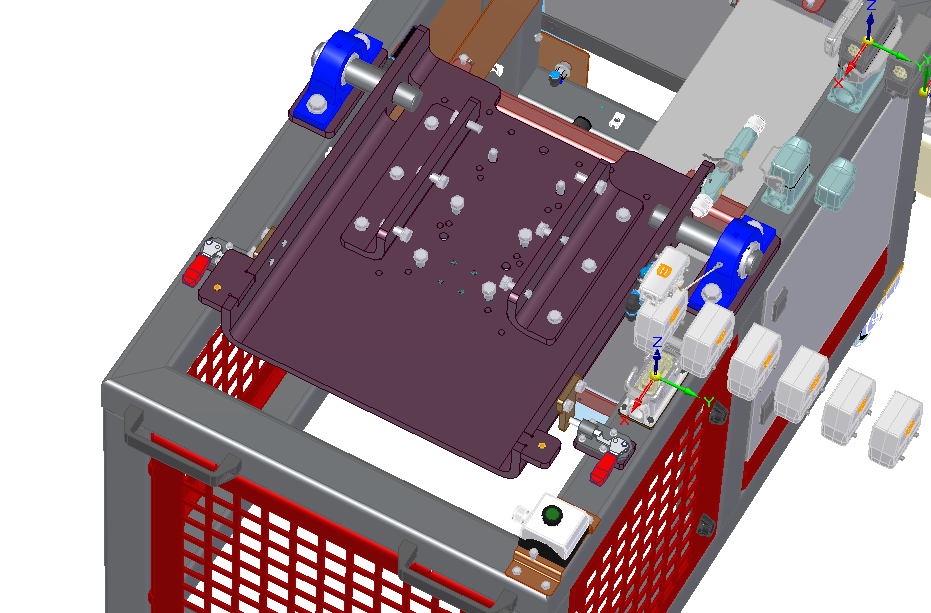
\includegraphics[width=\linewidth]{Foto3DModel}
	\caption{3D model mechanisch ontwerp}
	\label{fig:MechanischOntwerp}
\end{figure}

\begin{figure}[H]
	\centering
	\includegraphics[width=\linewidth]{Foto3DModel2}
	\caption{3D model mechanisch ontwerp met spindel}
	\label{fig:MechanischOntwerp2}
\end{figure}